\documentclass[conference]{IEEEtran}
\IEEEoverridecommandlockouts
\usepackage[utf8]{inputenc}
\usepackage[T1]{fontenc}
\usepackage[brazil]{babel}
\usepackage{cite}
\usepackage{amsmath,amssymb,amsfonts}
\usepackage{graphicx}
\usepackage{booktabs}
\usepackage{textcomp}
\renewcommand{\IEEEkeywordsname}{Palavras-chave}
\def\BibTeX{{\rm B\kern-.05em{\sc i\kern-.025em b}\kern-.08em T\kern-.1667em\lower.7ex\hbox{E}\kern-.125em X}}
\newcommand{\prodname}{\texttt{GLOBAL\_ANALYSISFORECAST\_PHY\_}\allowbreak\texttt{001\_024}}

\begin{document}

\title{Planejamento de Rota Marítima Inteligente com o Algoritmo A* e Dados Hidrodinâmicos Reais do Copernicus Marine Service}

\author{
\IEEEauthorblockN{Moisés Henrique Campanholo da Silva}
\IEEEauthorblockA{Engenharia da Computação\\
FHO -- Fundação Hermínio Ometto\\
Santa Cruz das Palmeiras, Brasil\\
RA: 114518\\
moiseshcs@alunos.fho.edu.br}
\and
\IEEEauthorblockN{Felipe Apolinário de Souza}
\IEEEauthorblockA{Engenharia da Computação\\
FHO -- Fundação Hermínio Ometto\\
Rio Claro, Brasil\\
RA: 114771\\
felipe.apolinario@alunos.fho.edu.br}
\and
\IEEEauthorblockN{Gabriel Vinícius Krebski}
\IEEEauthorblockA{Engenharia da Computação\\
FHO -- Fundação Hermínio Ometto\\
Artur Nogueira, Brasil\\
RA: 115442\\
gabriel.krebski@alunos.fho.edu.br}
}

\maketitle

\begin{abstract}
Este trabalho apresenta o desenvolvimento de um framework computacional baseado no algoritmo A* para o planejamento de rotas marítimas, utilizando dados hidrodinâmicos reais do Copernicus Marine Service. A motivação central é que a navegação que desconsidera o comportamento dinâmico das correntes oceânicas tende a gerar maior consumo de combustível, maiores emissões de gases de efeito estufa. O ambiente de navegação da Bacia de Santos (SP/RJ) é modelado como um grafo dirigido sobre a grade regular do produto \prodname, com máscara de terra extraída dos próprios dados NetCDF e vizinhança de 8 direções. O A* é adaptado com uma função de custo baseada no tempo de travessia, na qual a velocidade efetiva da embarcação incorpora a componente da corrente na direção do deslocamento, e com heurística admissível baseada na distância de Haversine. Uma segunda função de custo estima o consumo relativo de combustível, com velocidade sobre o fundo constante e consumo proporcional ao cubo da velocidade na água. A implementação foi desenvolvida em Python, com as bibliotecas xarray, pandas, NumPy, NetworkX e Matplotlib. A rota direta (linha reta), a rota A* de tempo e a rota A* de combustível são comparadas em um cenário de navegação costeira, em termos de tempo de travessia, consumo relativo de combustível, nós expandidos e mapas das rotas. Nos dados de 18/08/2026, a rota A* reduziu o consumo relativo de combustível em 3,17\% e o tempo de travessia em 1,03\% em relação à rota direta. Com as correntes reais, as rotas de tempo e de combustível coincidiram.
\end{abstract}

\begin{IEEEkeywords}
algoritmo A*, planejamento de trajetórias, correntes oceânicas, Copernicus Marine Service, grafo espacial, otimização de rotas, poluição marinha
\end{IEEEkeywords}

\section{Introdução}
O transporte marítimo e as atividades de exploração e gestão do oceano dependem diretamente das condições hidrodinâmicas locais --- correntes, ventos e variáveis biogeoquímicas --- para serem executados de forma eficiente e segura. Embarcações que navegam sem considerar o comportamento dinâmico da água tendem a percorrer trajetórias em linha reta ou baseadas exclusivamente na experiência do operador, ignorando informações públicas que poderiam tornar o deslocamento mais eficiente.

\subsection{Motivação: Consequências Práticas}
A ausência de sistemas de planejamento de rotas com dados oceanográficos reais gera problemas concretos e recorrentes:
\begin{itemize}
\item \textbf{Maior consumo de combustível e emissões de carbono:} navegar contra as correntes exige maior esforço do motor. Segundo a Organização Marítima Internacional (IMO), o transporte marítimo responde por $\approx$ 2,89\% das emissões globais de CO$_2$, e a otimização de rotas é apontada como estratégia direta para reduzir essa intensidade \cite{imo};
\item \textbf{Dispersão descontrolada de resíduos plásticos:} sem o mapeamento de zonas de convergência de correntes, embarcações de limpeza realizam varreduras ineficientes, cobrindo áreas de baixa concentração em vez de priorizar os pontos de maior acúmulo \cite{unep}.
\end{itemize}
Um paralelo útil é o dos aplicativos de navegação terrestre (Google Maps, Waze), que recalculam rotas considerando o trânsito. Não existe, de forma acessível, um equivalente para a navegação marítima que integre dados oceanográficos públicos a algoritmos de planejamento --- lacuna que este trabalho busca explorar.

\subsection{Relevância e Justificativa}
A relevância deste trabalho decorre da convergência de três fatores: (i) a disponibilidade pública e gratuita de dados oceanográficos de alta qualidade pelo Copernicus Marine Service, historicamente subutilizados em aplicações práticas de IA; (ii) a existência de problemas reais e documentados --- ambientais, econômicos e de segurança --- relacionados à ineficiência do planejamento de trajetórias marítimas \cite{imo,unep}; e (iii) a adequação do algoritmo A* \cite{hart}, consolidado na literatura de busca heurística, para incorporar informações físicas do ambiente em sua função de custo, produzindo soluções computacionalmente eficientes e completamente rastreáveis, o que é desejável em aplicações ligadas à segurança da navegação.

Ao utilizar exclusivamente dados públicos e institucionais como base experimental, o trabalho atende ao critério do roteiro da disciplina que atribui maior peso a problemas derivados de fontes reais e verificáveis.

\subsection{Objetivos}
\textbf{Objetivo geral:} desenvolver e avaliar um framework computacional baseado no algoritmo A*, adaptado para dados hidrodinâmicos reais, capaz de gerar rotas marítimas eficientes aplicáveis a cenários de navegação na Bacia de Santos (SP/RJ).

\textbf{Objetivos específicos:}
\begin{itemize}
\item Obter e tratar dados oceanográficos reais do Copernicus Marine Service para a região da Bacia de Santos;
\item Modelar a área marítima como grafo espacial bidimensional, com máscara de terra derivada automaticamente dos próprios dados NetCDF;
\item Adaptar a função de custo do A* para incorporar o campo vetorial de correntes, penalizando deslocamentos contrários ao fluxo e proibindo travessias de terra;
\item Implementar o A* com fila de prioridade do tipo min-heap e heurística admissível, obtendo a rota de menor custo no grafo discretizado, com meta de tempo de resposta interativo (inferior a 2 s por consulta);
\item Adaptar o custo do A* a um modelo de consumo relativo de combustível (velocidade sobre o fundo constante e consumo proporcional ao cubo da velocidade na água), como alternativa ao custo de tempo;
\item Avaliar comparativamente a rota direta (linha reta), a rota A* de tempo e a rota A* de combustível, em termos de tempo de travessia e de consumo relativo de combustível;
\end{itemize}

\subsection{Escopo}
Para garantir a viabilidade do projeto no prazo da disciplina, o trabalho é delimitado da seguinte forma: a área de estudo é a Bacia de Santos, com dados de 18 a 20 de agosto de 2026; a navegação é considerada apenas em superfície (nível de profundidade de 0,494 m), em um plano bidimensional; a única forçante física considerada são as correntes oceânicas (componentes $u_o$ e $v_o$), sem vento, ondas, batimetria, tráfego ou regras de navegação; o campo de correntes é tratado como estático durante cada consulta; a embarcação possui velocidade própria constante em relação à água; o consumo de combustível é uma estimativa relativa, sem calibração com dados de uma embarcação real; e o destino é um ponto fixo.

\subsection{Organização do Artigo}
A Seção II discute os trabalhos relacionados e posiciona a contribuição deste trabalho. A Seção III descreve a metodologia: definição do problema, dados, pré-processamento, modelagem em grafo, função de custo, heurística, ferramentas e processo de desenvolvimento e validação. A Seção IV apresenta os resultados da comparação entre a rota A* e a rota direta. A Seção V apresenta a conclusão e as limitações.

\section{Trabalhos Relacionados}
Esta seção organiza a literatura consultada em dois grupos: (i) algoritmos de busca e planejamento de trajetórias, que fornecem a técnica central do projeto; e (ii) caracterização física da região de estudo, que fornece a referência para interpretar os dados utilizados.

\subsection{Busca Heurística e o Algoritmo A*}
Hart, Nilsson e Raphael \cite{hart} abordam o problema de encontrar caminhos de custo mínimo em grafos. A técnica proposta, o A*, ordena a expansão dos nós pela função $f(n) = g(n) + h(n)$, combinando o custo acumulado $g(n)$ com uma estimativa $h(n)$ do custo restante. A principal contribuição do trabalho é a base formal que estabelece as condições sob as quais o algoritmo garante encontrar a solução ótima --- em especial, a exigência de que a heurística não superestime o custo real (admissibilidade). Para este projeto, esse resultado é central: como o custo de cada deslocamento varia com a direção da corrente, a heurística precisa ser construída de modo a continuar admissível, o que é discutido na Seção III-H.

\subsection{Planejamento de Trajetórias em Veículos Autônomos}
LaValle et al. \cite{lavalle} apresentam uma revisão de algoritmos de planejamento de trajetórias para veículos autônomos, organizando famílias de métodos como busca em grafos, métodos baseados em amostragem e abordagens de otimização. Segundo a revisão, a busca em grafos, da qual o A* faz parte, serve de base para sistemas que precisam lidar com custos direcionais variáveis. A contribuição do trabalho é sistematizar as vantagens e limitações de cada família conforme o tipo de ambiente. Para este projeto, a revisão orienta a escolha da técnica: como os dados do Copernicus já são fornecidos em uma grade regular, a discretização em grafo é natural, e a busca em grafos oferece determinismo e otimalidade na discretização, enquanto métodos de amostragem são mais adequados a espaços contínuos de alta dimensão.

\subsection{Pathfinding em Jogos}
Pardede et al. \cite{pardede} revisam algoritmos de pathfinding aplicados ao desenvolvimento de jogos, domínio em que agentes precisam encontrar caminhos em mapas discretizados (grids) com restrições de tempo real. A contribuição do trabalho é comparar algoritmos como A*, Dijkstra e suas variantes quanto à eficiência em mapas discretos. A relação com este projeto é direta: a grade oceânica, com células navegáveis e células de terra bloqueadas, é estruturalmente equivalente a um mapa de jogo com obstáculos. A diferença é que, aqui, o custo de cada movimento não é uniforme nem simétrico, pois depende de um campo físico real.

\subsection{Caracterização da Circulação na Região de Estudo}
Stramma e England \cite{stramma} descrevem as massas de água e a circulação média do Atlântico Sul, incluindo a Corrente do Brasil, que flui ao longo da margem continental sudeste brasileira. Embora não seja um trabalho de IA, ele fornece a referência física necessária para interpretar o campo de correntes utilizado (Fig.~\ref{fig:correntes}) e verificar qualitativamente a coerência dos dados antes de usá-los como custo no A*.

\subsection{Discussão Comparativa}
Comparando os trabalhos discutidos, observa-se que cada um contribui com uma parte diferente do problema, mas nenhum o resolve por completo. Hart et al. \cite{hart} oferecem a base formal do A* e a garantia de otimalidade com heurística admissível, mas pressupõem custos estáticos e conhecidos e um destino fixo. As revisões de LaValle et al. \cite{lavalle} e de Pardede et al. \cite{pardede} mostram a eficiência da busca em grafos em mapas discretos com obstáculos e justificam a escolha dessa família de métodos; porém, a primeira não trata dados oceanográficos, e a segunda considera custos geralmente uniformes, sem relação com fenômenos físicos reais.

Por fim, Stramma e England \cite{stramma} descrevem com rigor físico a circulação do Atlântico Sul e a Corrente do Brasil, servindo de referência para a validação qualitativa dos dados, mas não abordam o planejamento de rotas.

Em síntese, a busca heurística oferece otimalidade na discretização, determinismo e rastreabilidade da decisão, e a oceanografia física oferece a descrição do ambiente. Nos trabalhos de planejamento revisados, o custo do movimento é, em geral, tratado de forma abstrata (distância, obstáculos, terreno), sem estar associado a um campo vetorial físico real. Nos trabalhos oceanográficos, por outro lado, não há planejamento de rotas. Este projeto se situa na interseção entre esses dois grupos.

\subsection{Posicionamento e Diferencial: o que este trabalho faz de diferente?}
Considerando a literatura revisada, o diferencial deste trabalho está na combinação dos seguintes elementos:
\begin{enumerate}
\item \textbf{Custo derivado de um campo físico real:} o custo de cada aresta não é uma distância abstrata, mas o tempo de travessia calculado a partir da velocidade efetiva da embarcação, que incorpora as correntes do Copernicus. Com isso, o custo passa a ser dependente da direção ($c(u,v) \neq c(v,u)$);
\item \textbf{Máscara de terra obtida dos próprios dados:} o contorno costeiro é definido pela ausência de valores de corrente no arquivo NetCDF, dispensando shapefiles externos;
\item \textbf{Heurística admissível mesmo com custos direcionais:} a heurística usa uma velocidade superior a qualquer velocidade efetiva possível no domínio, preservando a garantia de otimalidade do A* \cite{hart} no grafo discretizado;
\item \textbf{Aplicação regional com dados institucionais públicos:} o método é aplicado à Bacia de Santos com dados gratuitos e verificáveis.
\end{enumerate}
Ao contrário de abordagens baseadas em aprendizado profundo, a busca heurística clássica é mantida como núcleo de decisão, de modo que cada rota gerada pode ser rastreada e explicada pela soma dos custos de suas arestas.

\section{Metodologia}
\subsection{Definição do Problema}
Dada uma grade oceânica regular com campo de correntes conhecido, uma célula de origem $s$ e uma célula de destino $t$, ambas navegáveis, deseja-se encontrar a rota $P = (s = n_0, n_1, \ldots, n_k = t)$ que minimiza o tempo total de travessia:
\begin{equation}
T(P) = \sum_{i=0}^{k-1} c(n_i, n_{i+1}),
\label{eq:T}
\end{equation}
em que $c(u,v)$ é o tempo de travessia da aresta $(u,v)$ (Eq.~\ref{eq:c}), sujeito às restrições: (i) todas as células da rota são navegáveis; (ii) movimentos diagonais não cortam terra; e (iii) nenhuma aresta é percorrida com velocidade efetiva igual ou inferior a 0,1 km/h. As hipóteses adotadas são as definidas no Escopo (Seção I-D). De forma análoga, o problema de combustível consiste em minimizar o consumo relativo $C(P) = \sum_{i=0}^{k-1} c_{comb}(n_i, n_{i+1})$ (Eq.~\ref{eq:ccomb}), sujeito às mesmas restrições.

\subsection{Visão Geral do Processo}
O experimento é organizado nas seguintes etapas, detalhadas nas subseções seguintes: (1) aquisição do recorte de dados no Copernicus Marine Service; (2) leitura do arquivo NetCDF e conversão para formato tabular; (3) correção dos campos de índice e cálculo da magnitude e da direção das correntes; (4) geração da máscara de terra e montagem das matrizes da grade; (5) construção do grafo dirigido de navegação; (6) execução do A* adaptado entre origem e destino; e (7) cálculo do tempo de travessia e comparação com a rota direta.

\subsection{Fonte e Características dos Dados}
Os dados são obtidos do produto \textit{Global Ocean Physics Analysis and Forecast} (\prodname), disponibilizado gratuitamente pelo Copernicus Marine Service --- serviço oficial de monitoramento oceânico da União Europeia, construído a partir de observações de satélite e modelagem numérica com assimilação de dados. A Fig.~\ref{fig:copernicus} mostra a interface de seleção do produto e das variáveis de interesse.

\begin{figure}[t]
\centering
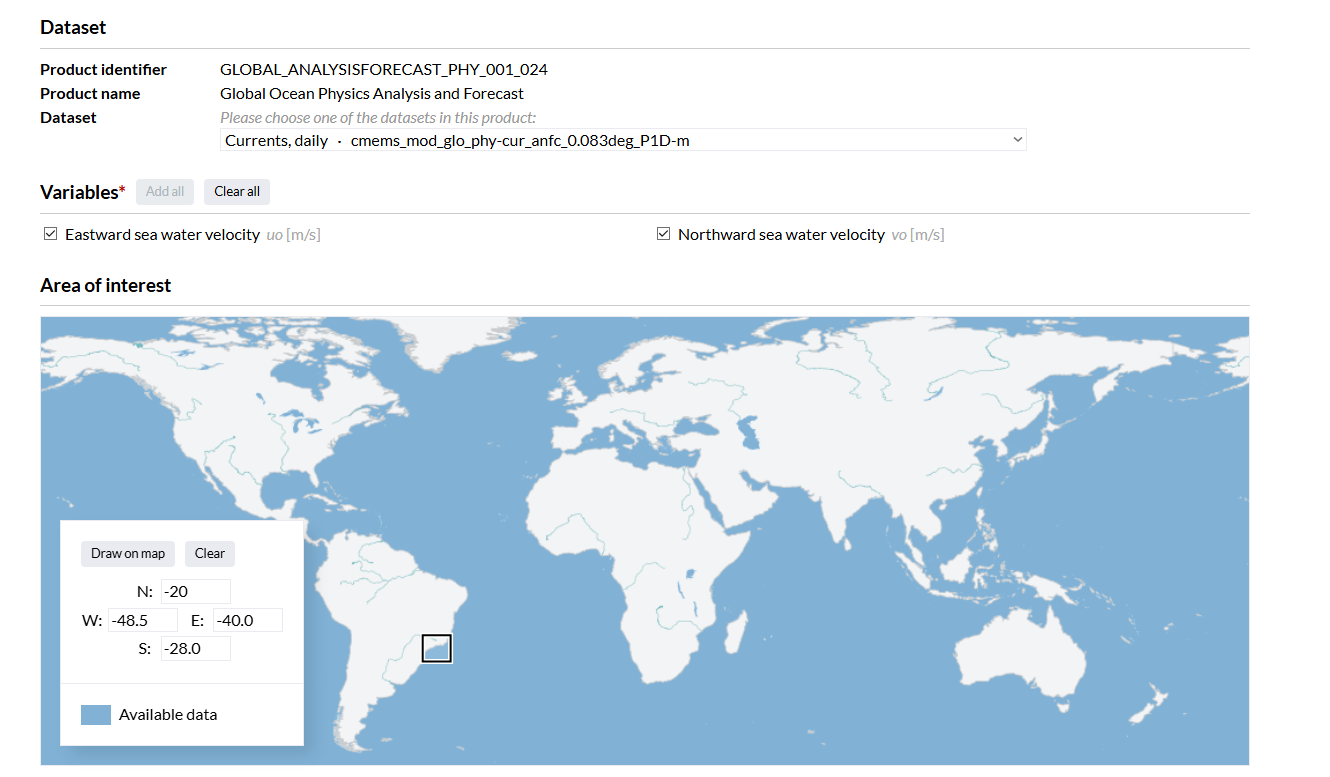
\includegraphics[width=\columnwidth]{fig1_copernicus.png}
\caption{Interface do Copernicus Marine Service para seleção do produto \prodname, com a área de interesse no litoral sudeste do Brasil e as variáveis $u_o$ e $v_o$ (m/s).}
\label{fig:copernicus}
\end{figure}

O conjunto de dados utilizado é o de correntes médias diárias (\texttt{cmems\_mod\_glo\_phy-cur\_anfc\_0.083deg\_P1D-m}), produzido pela Mercator Ocean International a partir do sistema global GLO12 e obtido no formato NetCDF (.nc) pelo Marine Data Store do Copernicus. O recorte possui resolução espacial de $1/12^\circ$ ($\approx 0{,}083^\circ$) e resolução temporal diária, com quatro dimensões: tempo (3 instantes, correspondentes aos dias 18, 19 e 20 de agosto de 2026), profundidade (um único nível, a 0,494 m, correspondente à superfície), latitude (49 pontos, de $-26^\circ$ a $-22^\circ$) e longitude (48 pontos, de $-47^\circ$ a $-43{,}08^\circ$). As variáveis extraídas são $u_o$, a componente zonal (leste--oeste) da velocidade da corrente, e $v_o$, a componente meridional (norte--sul), ambas em m/s.

A magnitude da corrente em cada célula é calculada como:
\begin{equation}
|\vec{V}| = \sqrt{u_o^2 + v_o^2}.
\label{eq:mag}
\end{equation}

A Fig.~\ref{fig:correntes} apresenta o campo vetorial das correntes na Bacia de Santos. Observa-se um núcleo de alta velocidade ($> 0{,}5$ m/s) na porção centro-leste, coerente com a posição da Corrente do Brasil descrita na literatura \cite{stramma}. É esse tipo de informação que a modelagem em grafo incorpora ao espaço de busca do A*.

\begin{figure}[t]
\centering
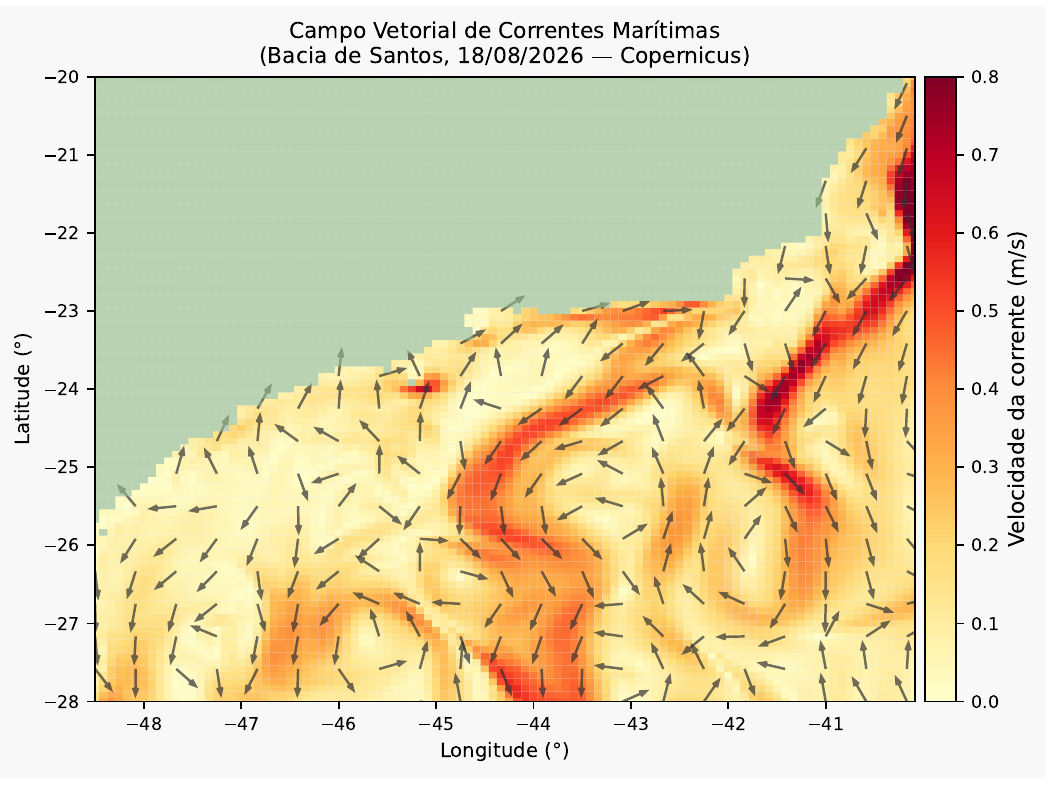
\includegraphics[width=\columnwidth]{fig2_correntes.png}
\caption{Campo vetorial e magnitude das correntes marítimas na Bacia de Santos (18/08/2026), obtido do Copernicus Marine Service. Setas indicam a direção do fluxo; cores indicam a intensidade (m/s).}
\label{fig:correntes}
\end{figure}

\subsection{Pré-processamento}
O arquivo NetCDF é lido com a biblioteca xarray e convertido em uma tabela (\textit{DataFrame}) da biblioteca pandas, com as colunas tempo, profundidade, latitude, longitude, $u_o$ e $v_o$. A tabela é exportada para uma planilha (.xlsx) e novamente carregada para o tratamento. Nessa conversão, os valores de tempo, profundidade e latitude aparecem apenas na primeira linha de cada grupo; por isso, essas três colunas são preenchidas por preenchimento sequencial (\textit{forward fill}). O preenchimento é aplicado somente a essas colunas de índice, e não às variáveis $u_o$ e $v_o$.

Em seguida, calculam-se para cada linha a magnitude da corrente (Eq.~\ref{eq:mag}) e a sua direção, $\theta = \operatorname{atan2}(v_o, u_o)$, em radianos. As células sem leitura válida de corrente correspondem a áreas de continente ou ilhas e são marcadas como bloqueadas (\texttt{is\_land = True}). Essa abordagem dispensa o uso de \textit{shapefile} externo, pois a própria ausência de dados do Copernicus delimita o contorno costeiro.

Por fim, os dados de um instante de tempo são reorganizados em matrizes: as latitudes e longitudes distintas são ordenadas e mapeadas para índices de linha $r$ e coluna $c$, e são criadas as matrizes $u_o[r,c]$, $v_o[r,c]$ e \texttt{is\_land}$[r,c]$. Todas as células começam marcadas como terra e passam a água apenas quando possuem valores válidos de $u_o$ e $v_o$.

\subsection{Modelagem do Ambiente em Grafo}
A área marítima é modelada como um grafo dirigido $G = (V, E)$, construído explicitamente com a classe \texttt{DiGraph} da biblioteca NetworkX, conforme o seguinte processo:
\begin{enumerate}
\item \textbf{Nós:} percorre-se toda a grade e, para cada célula $(r,c)$ com \texttt{is\_land = False}, é criado um nó identificado por $(r,c)$ e associado à sua posição geográfica (latitude, longitude). Células de terra não geram nós e, portanto, não participam de nenhuma aresta;
\item \textbf{Vizinhança:} para cada nó, são examinados os 8 vizinhos possíveis (4 ortogonais e 4 diagonais). Um vizinho só é considerado se também for um nó do grafo, isto é, se for água e estiver dentro dos limites da grade;
\item \textbf{Restrição diagonal:} um movimento diagonal só é permitido se as duas células ortogonais intermediárias forem navegáveis, evitando cortes por penínsulas ou ilhas;
\item \textbf{Pesos:} para cada par válido, calcula-se o tempo de travessia $c(u,v)$ (Eq.~\ref{eq:c}) e cria-se a aresta dirigida $(u,v)$ com esse peso. Arestas de custo infinito não são adicionadas.
\end{enumerate}
Formalmente, o conjunto de arestas é:
\begin{multline}
E = \{(u,v) : u,v \in V,\ v \in N_8(u), \text{ e, se diagonal,}\\
(r_u, c_v) \in V \wedge (r_v, c_u) \in V\}.
\label{eq:E}
\end{multline}
O grafo é dirigido porque o custo de percorrer uma aresta depende do sentido do movimento em relação à corrente; em geral, $c(u,v) \neq c(v,u)$.

A Fig.~\ref{fig:grafo} mostra o grafo gerado pela implementação em uma grade de teste com as mesmas dimensões da grade real ($49 \times 48$ células), utilizada para verificar a construção dos nós, das arestas e da máscara de terra.

\begin{figure}[t]
\centering
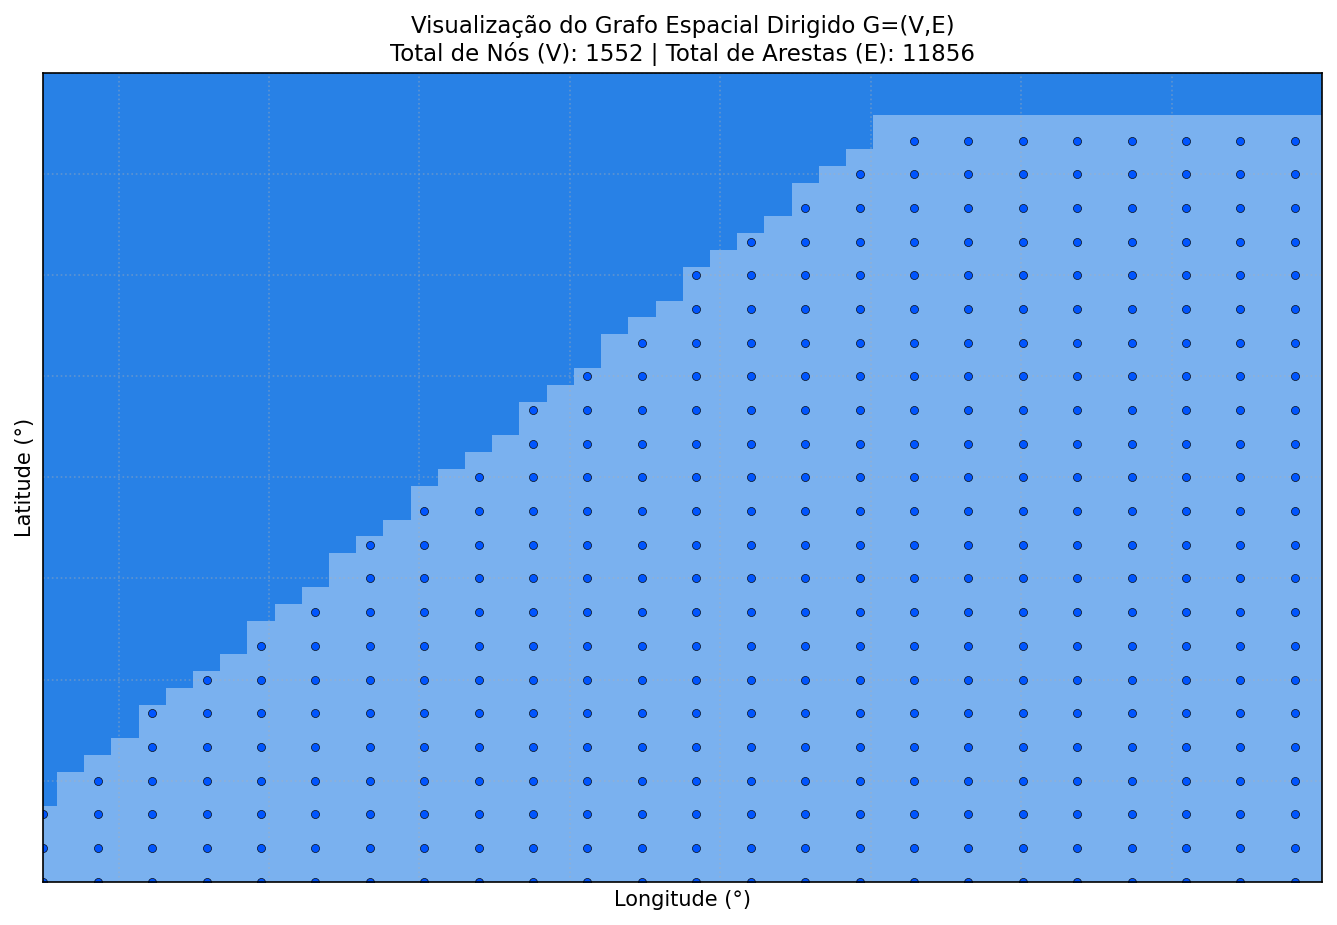
\includegraphics[width=\columnwidth]{fig3_grafo.png}
\caption{Grafo espacial dirigido $G = (V,E)$ gerado pela implementação em uma grade de teste de $49 \times 48$ células com máscara de terra sintética (1552 nós e 11856 arestas). A área em azul-escuro corresponde à terra e a área clara ao oceano. Para legibilidade, é exibido um a cada dois nós em cada direção.}
\label{fig:grafo}
\end{figure}

\subsection{Justificativa da Escolha do A*}
O A* foi escolhido por quatro motivos. Primeiro, os dados do Copernicus já são fornecidos em grade regular, o que torna natural a representação discreta em grafo, cenário em que a busca em grafos é a família de métodos indicada \cite{lavalle,pardede}. Segundo, com heurística admissível, o A* encontra a mesma solução ótima que o algoritmo de Dijkstra, mas tende a expandir menos nós, por direcionar a busca ao destino \cite{hart}. Terceiro, métodos baseados em amostragem, como o RRT, são mais adequados a espaços contínuos de alta dimensão e não garantem otimalidade em tempo finito, o que não se justifica em uma grade bidimensional. Quarto, o A* não requer dados de treinamento e produz decisões determinísticas e rastreáveis.

\subsection{Função de Custo}
O A* minimiza $f(n) = g(n) + h(n)$, em que $g(n)$ é o custo acumulado desde a origem e $h(n)$ é a heurística. O custo de cada aresta incorpora as correntes pela velocidade efetiva da embarcação sobre o fundo:
\begin{equation}
v_{ef}(u,v) = v_{navio} + \vec{V}_{corrente} \cdot \hat{u}_{uv},
\label{eq:vef}
\end{equation}
em que $v_{navio} = 18{,}5$ km/h é a velocidade própria da embarcação; $\vec{V}_{corrente} = 3{,}6\,(v_o, u_o)$ é a corrente da célula de origem $u$, convertida de m/s para km/h e expressa nas componentes norte e leste; e $\hat{u}_{uv} = (\Delta\varphi, \Delta\lambda)/\lVert(\Delta\varphi, \Delta\lambda)\rVert$ é o vetor unitário do rumo, obtido pelas diferenças de latitude e longitude entre os centros das células $u$ e $v$. Uma corrente favorável aumenta $v_{ef}$; uma corrente contrária a reduz.

O custo (tempo de travessia, em horas) da aresta é:
\begin{equation}
c(u,v) =
\begin{cases}
\dfrac{d_H(u,v)}{v_{ef}(u,v)}, & \text{se } v_{ef}(u,v) > 0{,}1 \text{ km/h},\\[2mm]
\infty, & \text{caso contrário,}
\end{cases}
\label{eq:c}
\end{equation}
em que $d_H(u,v)$ é a distância de Haversine, em km, entre os centros das células:
\begin{multline}
d_H(a,b) = 2R \arcsin\!\sqrt{\sin^2\tfrac{\Delta\varphi}{2} + \cos\varphi_a \cos\varphi_b \sin^2\tfrac{\Delta\lambda}{2}},
\end{multline}
com $\varphi$ e $\lambda$ em radianos e $R = 6371$ km (raio médio da Terra). O custo acumulado é atualizado por $g(v) = g(u) + c(u,v)$, e o custo total de uma rota é o seu tempo de travessia $T(P)$ (Eq.~\ref{eq:T}).

\textit{Custo de combustível.} Com velocidade própria constante na água, o consumo é proporcional ao tempo e não distinguiria as rotas. Por isso, o modelo de combustível adota velocidade \emph{sobre o fundo} constante ($v_{navio}$), com o motor compensando a corrente, e a aproximação usual de que a potência de propulsão --- e, portanto, o consumo por hora --- cresce com o cubo da velocidade na água \cite{psaraftis}. A velocidade na água necessária em cada aresta é
\begin{equation}
v_{agua}(u,v) = v_{navio} - \vec{V}_{corrente} \cdot \hat{u}_{uv},
\label{eq:vagua}
\end{equation}
e o consumo relativo da aresta, em unidades relativas (u.r.), é:
\begin{equation}
c_{comb}(u,v) =
\begin{cases}
\dfrac{d_H(u,v)}{v_{navio}}\left(\dfrac{v_{agua}(u,v)}{v_{navio}}\right)^{3}, & \text{se } v_{agua}(u,v) > 0{,}1 \text{ km/h},\\[2mm]
\infty, & \text{caso contrário.}
\end{cases}
\label{eq:ccomb}
\end{equation}
Uma unidade relativa equivale a 1 h de navegação em água parada à velocidade de cruzeiro; uma rota de $L$ km em água parada consumiria $L/v_{navio}$ u.r. Corrente a favor reduz $v_{agua}$ e o consumo; corrente contrária os aumenta.

\subsection{Heurística}
A heurística é a distância de Haversine até o destino dividida por uma velocidade máxima fixa:
\begin{equation}
h(n) = \frac{d_H(n,t)}{v_{max}}, \qquad v_{max} = 25 \text{ km/h}.
\label{eq:h}
\end{equation}
\textit{Admissibilidade:} pela Eq.~\ref{eq:vef}, a velocidade efetiva de qualquer aresta é no máximo $v_{navio} + 3{,}6\,|\vec{V}|$. Assim, $v_{ef} \leq v_{max}$ sempre que $|\vec{V}| \leq (25 - 18{,}5)/3{,}6 \approx 1{,}8$ m/s, condição atendida pelo campo da Fig.~\ref{fig:correntes}, cujas magnitudes não ultrapassam cerca de 0,8 m/s. Nesse caso, $c(u,v) \geq d_H(u,v)/v_{max}$ e, pela desigualdade triangular na esfera, a soma das distâncias de qualquer rota de $n$ até $t$ é maior ou igual a $d_H(n,t)$. Portanto, $h(n)$ nunca superestima o custo real e, pelo mesmo argumento, $h(u) \leq c(u,v) + h(v)$ (consistência). Pelo resultado de Hart et al. \cite{hart}, o A* retorna a rota de menor tempo de travessia no grafo $G$; essa otimalidade vale para a discretização adotada, e não para o espaço contínuo.

Para o critério de combustível, a heurística é a distância de Haversine até o destino multiplicada pelo menor consumo por km possível:
\begin{equation}
h_{comb}(n) = \frac{d_H(n,t)}{v_{navio}}\left(\frac{v_{navio} - 3{,}6\,V_{max}}{v_{navio}}\right)^{3}, \qquad V_{max} = 0{,}8 \text{ m/s}.
\label{eq:hcomb}
\end{equation}
Como $v_{agua} \geq v_{navio} - 3{,}6\,|\vec{V}|$ e $|\vec{V}| \leq V_{max}$ nos dados utilizados, cada aresta custa ao menos $d_H(u,v)$ vezes o fator da Eq.~\ref{eq:hcomb}; pelo mesmo argumento da desigualdade triangular, $h_{comb}$ é admissível e consistente. A condição $|\vec{V}| \leq V_{max}$ é verificada no código para cada instante.

\subsection{Execução do A*}
A busca é realizada por uma implementação própria do A* em Python, com fila de prioridade do tipo \textit{min-heap} binária (módulo \texttt{heapq}), com custo $O(\log n)$ por operação de inserção e remoção. A mesma rotina atende aos dois critérios: com o peso de tempo (Eq.~\ref{eq:c}) e a heurística da Eq.~\ref{eq:h}, obtém-se a rota A* de tempo; com o peso de combustível (Eq.~\ref{eq:ccomb}) e a heurística da Eq.~\ref{eq:hcomb}, a rota A* de combustível. A implementação registra o número de nós expandidos, isto é, retirados da fila e fechados; com $h(n) = 0$, a rotina equivale ao algoritmo de Dijkstra, usado como referência de custo computacional em cada critério. O custo da rota obtida é conferido, em todas as execuções, contra o da função \texttt{astar\_path} da biblioteca NetworkX, aplicada ao mesmo grafo e à mesma heurística. O custo total de uma rota é a soma dos pesos de suas arestas.

\subsection{Ferramentas, Linguagem e Bibliotecas}
O projeto foi desenvolvido na linguagem Python, em ambiente Jupyter Notebook. As bibliotecas utilizadas e suas funções no projeto são: xarray, para a leitura do arquivo NetCDF; pandas, para a conversão em tabela, a exportação e leitura da planilha, o preenchimento sequencial dos índices e a tabulação dos resultados; NumPy, para as operações matriciais, a magnitude, a direção e a distância de Haversine; NetworkX, para a construção do grafo dirigido e a verificação do custo da rota com \texttt{astar\_path}; e Matplotlib, para as visualizações do campo de correntes, do grafo e das rotas. A biblioteca padrão \texttt{math} é usada no cálculo do vetor unitário do rumo, e os módulos \texttt{heapq} e \texttt{time}, na fila de prioridade da busca e na medição do tempo de execução.

\subsection{Processo de Desenvolvimento e Validação}
O desenvolvimento foi incremental, seguindo a ordem das etapas descritas na Seção III-B: primeiro, a leitura e a inspeção do arquivo NetCDF; depois, a conversão tabular e o pré-processamento; em seguida, a implementação das funções de distância, custo e heurística e a construção do grafo; e, por fim, a execução do A* e a visualização. A construção do grafo e a execução do A* foram inicialmente verificadas na grade de teste da Fig.~\ref{fig:grafo}, permitindo conferir visualmente que nenhuma aresta atravessa terra e que os movimentos diagonais respeitam a restrição da Eq.~\ref{eq:E}.

A validação do planejador compara as rotas obtidas pelo A* (tempo e combustível) com a rota direta (linha reta) entre os mesmos pontos de origem e destino, em termos de tempo total de travessia, consumo relativo de combustível, número de células percorridas e nós expandidos (A* $\times$ Dijkstra), em um estudo de caso de navegação costeira, com destino fixo.

\section{Resultados}
\subsection{Protocolo Experimental}
Os experimentos foram executados sobre o grafo da Seção III, construído com o campo de correntes de 18/08/2026 (1494 nós navegáveis na grade de $49 \times 48$ células). Foi avaliado o estudo de caso de navegação costeira da Seção III-K, com origem em ($-26{,}00^\circ$; $-47{,}00^\circ$) e destino em ($-22{,}92^\circ$; $-43{,}08^\circ$), nos extremos sudoeste e nordeste do recorte.

Comparam-se três rotas: a \textbf{rota direta}, formada pelas células amostradas sobre o segmento origem--destino; a \textbf{rota A* de tempo}, que minimiza a Eq.~\ref{eq:c}; e a \textbf{rota A* de combustível}, que minimiza a Eq.~\ref{eq:ccomb}. Como as três são sequências de células do mesmo grafo, cada uma é avaliada nos dois critérios: o tempo $T(P)$, pelo modelo de velocidade própria constante, e o consumo relativo $C(P)$, pelo modelo de velocidade sobre o fundo constante. Os dois modelos descrevem modos de operação distintos; a comparação é feita sobre os caminhos, e não sobre uma mesma viagem. Nenhuma aresta da rota direta atravessa terra, de modo que a comparação é válida. As métricas são: $T(P)$, $C(P)$ em u.r., comprimento (Haversine), células percorridas, nós expandidos (A* $\times$ Dijkstra no mesmo critério) e tempo de execução da busca (média de 30 execuções). Em todas as execuções, o A*, o Dijkstra e a função \texttt{astar\_path} da NetworkX retornaram o mesmo custo (diferença inferior a $10^{-9}$). O consumo é uma estimativa relativa, comparável entre rotas, sem calibração com uma embarcação real.

\subsection{Resultados Quantitativos}
A Tabela~\ref{tab:res} reúne as métricas do campo de 18/08/2026, e a Fig.~\ref{fig:mapa1} mostra as rotas sobre a magnitude das correntes.

\begin{table}[t]
\caption{Rota direta $\times$ A* de tempo $\times$ A* de combustível (campo de 18/08/2026).}
\label{tab:res}
\centering
\footnotesize
\begin{tabular}{@{}lccc@{}}
\toprule
Métrica & Direta & A* tempo & A* comb.\\
\midrule
Tempo (h) & 30,75 & 30,43 & 30,43\\
Combustível (u.r.) & 33,01 & 31,97 & 31,97\\
Comprimento (km) & 547,9 & 548,9 & 548,9\\
Células percorridas & 48 & 48 & 48\\
Nós expandidos & --- & 1264 & 1452\\
Nós expandidos (Dijkstra) & --- & 1494 & 1494\\
Tempo de busca (ms) & --- & 25,6 & 25,0\\
\bottomrule
\end{tabular}
\end{table}

\begin{figure}[t]
\centering
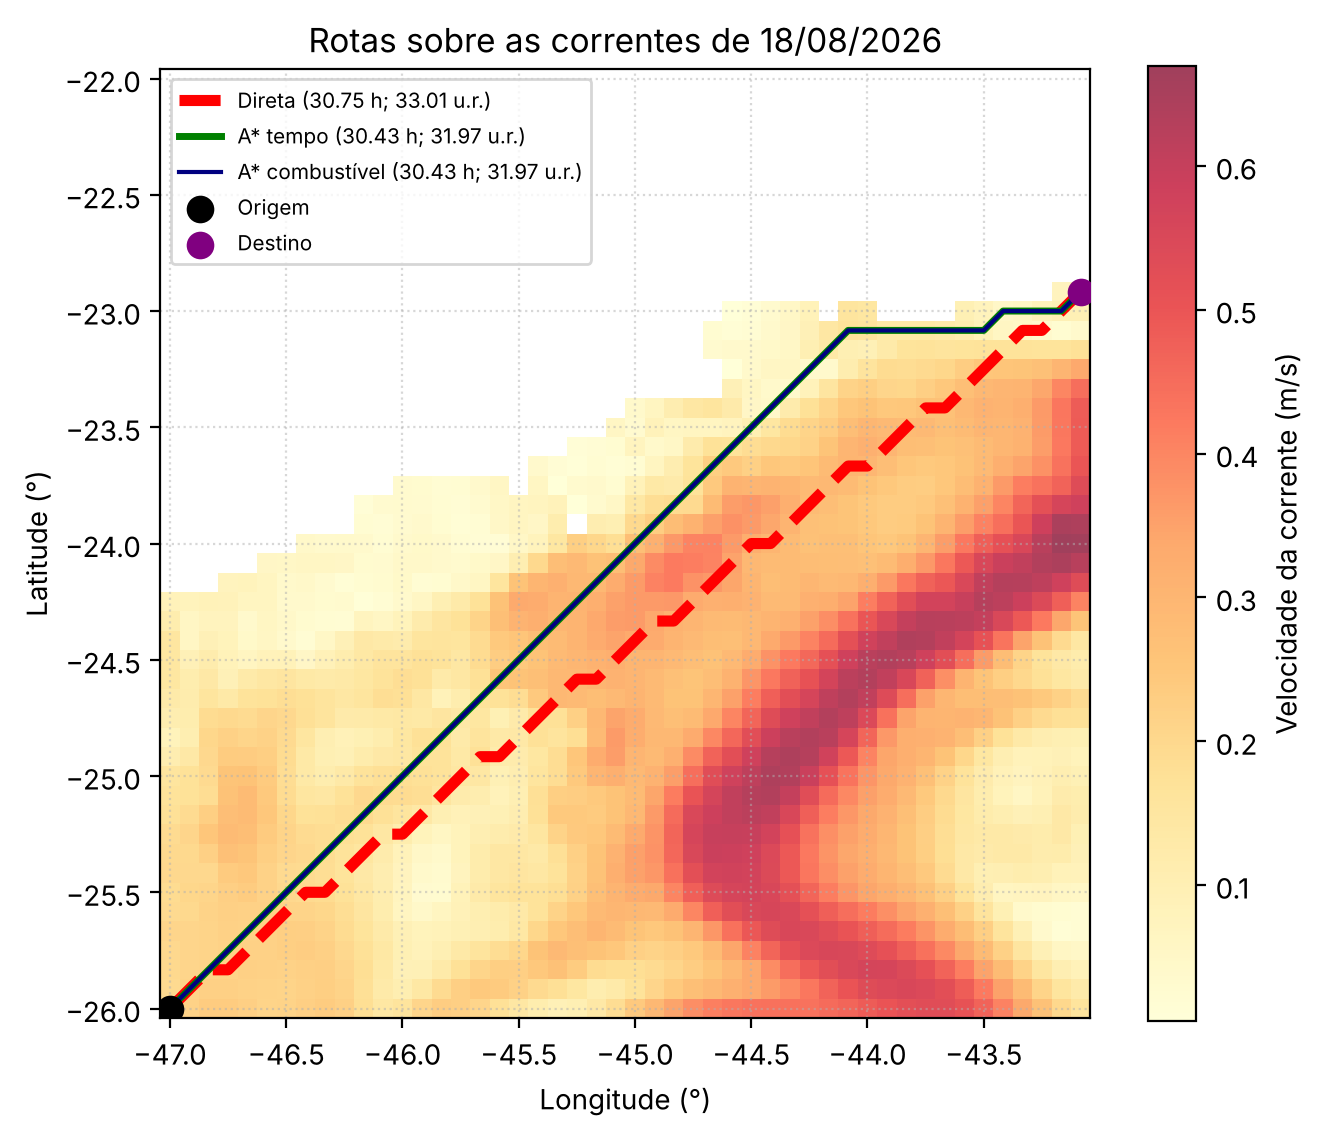
\includegraphics[width=\columnwidth]{mapa_rotas.png}
\caption{Rota direta (vermelho tracejado), rota A* de tempo (verde) e rota A* de combustível (azul), sobre a magnitude das correntes de 18/08/2026. As duas rotas A* coincidem.}
\label{fig:mapa1}
\end{figure}

Repetindo o experimento nos três dias do recorte, a redução de combustível em relação à rota direta foi de 3,17\% (18/08), 4,25\% (19/08) e 4,85\% (20/08), contra 1,03\%, 1,31\% e 1,49\% de redução de tempo. Os nós expandidos pelo A* de combustível foram 1452, 1291 e 1179, contra 1494 do Dijkstra em todos os dias.

\textit{Sensibilidade.} Com as correntes reais, a rota A* de combustível coincidiu com a A* de tempo em todos os casos. Para verificar quando o critério passa a alterar a rota, o experimento foi repetido com as correntes de 18/08 \emph{multiplicadas artificialmente} por um fator (Tabela~\ref{tab:sens}); como a heurística deixa de ser admissível com correntes ampliadas, essa análise usa o Dijkstra. Trata-se de um teste de sensibilidade do modelo, e não de um cenário real.

\begin{table}[t]
\caption{Sensibilidade: correntes de 18/08 multiplicadas por um fator (Dijkstra). Combustível em u.r., tempo em h.}
\label{tab:sens}
\centering
\footnotesize
\begin{tabular}{@{}cccccc@{}}
\toprule
Fator & $|\vec{V}|_{max}$ & Mesma & Comb. & Comb. & Tempo\\
 & (m/s) & rota? & direta & A* comb. & A* comb./tempo\\
\midrule
$\times$1 & 0,67 & sim & 33,01 & 31,97 & 30,43/30,43\\
$\times$3 & 2,01 & não & 40,77 & 33,98 & 32,81/32,19\\
$\times$6 & 4,02 & não & 55,05 & 35,99 & 33,89/33,56\\
\bottomrule
\end{tabular}
\end{table}

\subsection{Discussão}
A rota A* reduziu o consumo relativo de combustível em 3,17\% (33,01 para 31,97 u.r.) e o tempo em 1,03\% (0,32 h), mesmo percorrendo um caminho 0,17\% mais longo (548,9 km contra 547,9 km). Como mostra a Fig.~\ref{fig:mapa1}, a rota A* se afasta da reta em direção à região de menor intensidade de corrente, ao norte do eixo de maior velocidade. A redução de combustível é cerca de três vezes a de tempo porque a lei cúbica amplifica o efeito da corrente: a corrente máxima do campo de 18/08 ($\approx$ 0,67 m/s, ou 2,4 km/h) equivale a cerca de 13\% da velocidade de cruzeiro (18,5 km/h) e altera o consumo por hora em cerca de $+44\%$ (contra a corrente) ou $-34\%$ (a favor), enquanto o tempo varia em proporção bem menor. Nos três dias, as reduções ficaram entre 3,17\% e 4,85\% (combustível) e entre 1,03\% e 1,49\% (tempo).

\textbf{Combustível $\times$ tempo.} Com as correntes reais, as rotas A* de tempo e de combustível coincidiram nos três dias avaliados: para correntes de até cerca de 0,7 m/s, os dois critérios ordenam os caminhos da mesma forma, e minimizar o tempo já minimiza o consumo estimado. Na análise de sensibilidade (Tabela~\ref{tab:sens}), com correntes multiplicadas por 3 ($|\vec{V}|_{max}$ = 2,01 m/s), as rotas se separam: a de combustível consome 7,1\% menos que a de tempo (33,98 contra 36,58 u.r.), ao custo de 2,0\% mais tempo (32,81 contra 32,19 h), e 16,6\% menos que a rota direta. O critério de combustível só altera a rota, portanto, quando as correntes são suficientemente fortes.

\textbf{Custo computacional.} O A* de tempo expandiu 15,4\% menos nós que o Dijkstra, o que é consistente com o efeito esperado de uma heurística admissível \cite{hart}. O A* de combustível expandiu apenas 2,8\% menos: sua heurística (Eq.~\ref{eq:hcomb}) usa o menor consumo por km possível, cerca de 60\% do valor em água parada, e por isso é pouco informativa. O tempo de busca (25,6 ms para tempo e 25,0 ms para combustível, no ambiente de teste) ficou abaixo da meta de 2 s por consulta.

\textbf{Comparação com a literatura.} Os trabalhos revisados \cite{hart,lavalle,pardede,stramma,psaraftis} não reportam resultados comparáveis (rotas sob correntes reais do Copernicus com custo de tempo ou de combustível); por isso, a comparação quantitativa limita-se à rota direta e ao Dijkstra, definidos acima.

\section{Conclusão}
Este trabalho implementou um planejador de rotas marítimas baseado no A*, com dois critérios de custo calculados a partir das correntes do Copernicus Marine Service: o tempo de travessia e o consumo relativo de combustível, este com velocidade sobre o fundo constante e consumo proporcional ao cubo da velocidade na água. Nos dados de 18/08/2026, o grafo dirigido tem 1494 nós, e o A* retornou, em todas as execuções, o mesmo custo mínimo do Dijkstra.

\textbf{Principais resultados.} No estudo de caso costeiro, a rota A* reduziu o consumo relativo de combustível em 3,17\% (33,01 para 31,97 u.r.) e o tempo de travessia em 1,03\% (30,75 para 30,43 h) em relação à rota direta; nos três dias do recorte, as reduções de combustível ficaram entre 3,17\% e 4,85\%. As rotas A* de tempo e de combustível coincidiram com as correntes reais, e só se separaram na análise de sensibilidade com correntes ampliadas, em que a de combustível consumiu 7,1\% menos que a de tempo, com 2,0\% mais tempo. O A* expandiu 15,4\% menos nós que o Dijkstra com o custo de tempo e 2,8\% com o de combustível.

\textbf{Cumprimento dos objetivos.} A obtenção e o tratamento dos dados reais, a modelagem em grafo com máscara de terra extraída do NetCDF e as funções de custo de tempo e de combustível foram atingidos. O A* com fila de prioridade (min-heap) e heurísticas admissíveis também foi atingido, com 25,6 ms (tempo) e 25,0 ms (combustível) por consulta, abaixo da meta de 2 s. A avaliação comparativa com a rota direta foi realizada: as reduções medidas foram pequenas, de até 4,85\% em combustível e 1,49\% em tempo nos casos testados. O consumo de combustível é uma estimativa relativa de um modelo simplificado, sem calibração com dados de uma embarcação; não representa consumo medido nem emissões.

\textbf{Limitações.} Além das hipóteses simplificadoras --- (i) o campo de correntes é tratado como estático durante cada consulta; (ii) a navegação é restrita à superfície, em duas dimensões; (iii) a velocidade própria da embarcação é constante; (iv) a velocidade efetiva considera apenas a componente da corrente na direção do deslocamento, desprezando a deriva lateral; (v) vento, ondas e batimetria não são considerados; e (vi) a otimalidade é garantida apenas no grafo discretizado, cujas direções de movimento são limitadas às 8 da vizinhança adotada ---, o modelo de combustível adota a lei cúbica sem curva de consumo do motor, e os modelos de tempo e de combustível assumem modos de operação distintos (velocidade própria constante e velocidade sobre o fundo constante). Os resultados se restringem a um estudo de caso com um único par origem--destino; a três dias consecutivos de uma única região; à resolução de $1/12^\circ$ ($\approx$ 9 km); e a tempos de execução medidos em um único ambiente. A análise de sensibilidade usa correntes artificiais e não prevê o comportamento real. Não houve validação contra trajetórias ou consumo reais de embarcações.


\begin{thebibliography}{00}
\bibitem{imo} International Maritime Organization (IMO), ``Fourth IMO GHG Study 2020: Full Report,'' IMO, London, UK, 2020.
\bibitem{unep} United Nations Environment Programme (UNEP), ``From Pollution to Solution: a Global Assessment of Marine Litter and Plastic Pollution,'' 2021.
\bibitem{hart} P. E. Hart, N. J. Nilsson e B. Raphael, ``A formal basis for the heuristic determination of minimum cost paths,'' IEEE Trans. Systems Science and Cybernetics, vol. 4, n. 2, pp. 100--107, 1968.
\bibitem{lavalle} S. M. LaValle et al., ``A Survey of Autonomous Vehicle Behaviors: Trajectory Planning Algorithms,'' PMC/NCBI, 2024.
\bibitem{pardede} S. L. Pardede et al., ``A Review of Pathfinding in Game Development,'' ResearchGate, 2021.
\bibitem{stramma} L. Stramma e M. England, ``On the water masses and mean circulation of the South Atlantic Ocean,'' J. Geophysical Research: Oceans, vol. 104, n. C9, pp. 20863--20883, 1999.
\bibitem{psaraftis} H. N. Psaraftis e C. A. Kontovas, ``Speed models for energy-efficient maritime transportation: A taxonomy and survey,'' Transportation Research Part C: Emerging Technologies, vol. 26, pp. 331--351, 2013.
\end{thebibliography}

\end{document}
